
\begin{table}
  \centering
  \begin{tabular}{ l | c | r }
    \hline
    Model               & Encoding  & Accuracy \\
    \hline
    MLP                 & char bi-gram &  0.898 \\
    CNN                 & char bi-gram & \textbf{0.956} \\
    % LSTM                & char bi-gram & 60k & 0.933 \\
    MLP                 & char uni-gram &  0.697\\
    CNN                 & char uni-gram  & 0.942 \\
    % LSTM                & char uni-gram & 60k &  \\
    \hline
  \end{tabular}
  \caption{Overview of results for the neural network models for the data set with 10K data points in each language.}
  \label{keras-results}
\end{table}

\section{Results}

\subsection{Results with neural networks}
In the following we evaluate the initial results for the neural network architectures which can be seen in Table~\ref{keras-results}. Here we compare the result of doing character level uni- and bi-grams using the Multilayer Perceptron and Convolutional Neural Network. We see that the CNN performs the best, achieving an accuracy of 95.6\% when using character bi-grams. Both models perform better using bi-grams than individual characters as features while the relative increase in performance is greater for the MLP model.\\


\subsection{Increasing the size of the data set}
Usually the performance of supervised classification models increase with more training data. To measure this effect we increase the amount of training data to 50K sentences in each of the language categories. Due to much longer training times only the "baseline models" are included with the skip-gram encoding from FastText which we saw achieved the highest accuracy.\\ 

\begin{table}
  \centering
  \begin{tabular}{ l  c | r }
    \hline
    Model               & Encoding & Accuracy \\
    \hline
    Knn                 & skipgram & 0.931\\
    Logistic Regression & skipgram  & \textbf{0.933}\\
    Naive Bayes         & skipgram  & 0.806\\
    SVM                 & skipgram& 0.925\\
    \hline
  \end{tabular}
  \caption{Overview of results for the data set with 50K data points in each language.}
  \label{results-sklearn300k}
\end{table}


\begin{table}
  \centering
  \begin{tabular}{ l c | r }
    \hline
    Model               & Encoding & Accuracy \\
    \hline
    MLP                 & char bi-gram  & 0.918\\
    CNN                 & char bi-gram  & \textbf{0.970}\\
    \hline
  \end{tabular}
  \caption{Overview of results for the data set with 50K data points in each language.}
  \label{results-keras-300k}
\end{table}

Table~\ref{results-sklearn300k} show that the accuracies for the logistic regression model and the K nearest neighbors algorithm improved slightly by including more data. Unexpectedly, performance of the support vector machine and naive Bayes dropped a bit with extra data.\\

Even when including five times the amount of data the best result, logistic regression with an accuracy of 93.3\%, is still worse than for the Convolutional Neural Network trained on 10K data points in each language.\\

In Table~\ref{results-keras-300k} we see the results for running the neural networks on the larger data set. Both models improve by increasing the amount of data and the Convolutional Neural Network reached an accuracy of 97\% which is the best so far.\\


\begin{figure}
  \centering
  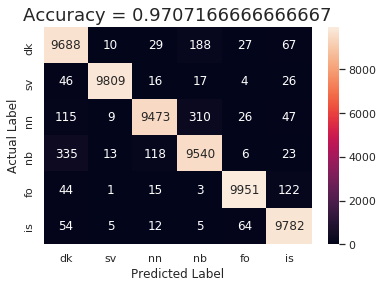
\includegraphics[scale=0.5]{figs/confusion_CNN}
  \caption{Confusion matrix with results from the convolutional neural network on the full data set with 50K data points in each language.}
  \label{confusion_matrix-big-cnn}
\end{figure}

\begin{figure}
  \centering
  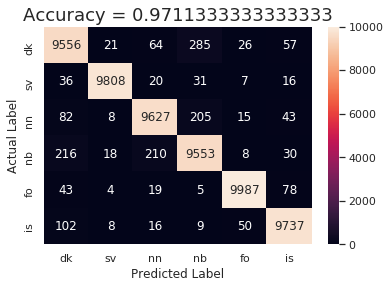
\includegraphics[scale=0.5]{figs/fasttext_supervised}
  \caption{Confusion matrix with results from a supervised FastText model on the full data set with 300K data points.}
  \label{fasttext_supervised}
\end{figure}

\begin{figure}
    \centering
    \begin{subfigure}[b]{0.45\textwidth}
      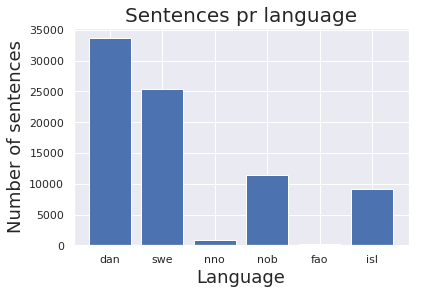
\includegraphics[scale=0.5]{figs/tatoebasentprlang}
      \caption{Distribution of the number of sentences in each language in the Tatoeba data set.}
      \label{tatoebasentprlang}
    \end{subfigure}
    ~
    \begin{subfigure}[b]{0.45\textwidth}
      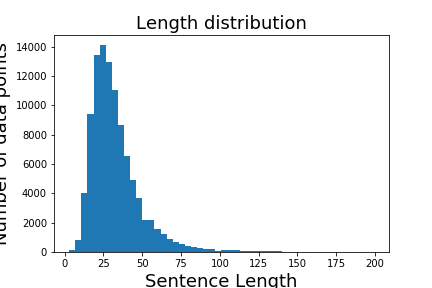
\includegraphics[scale=0.5]{figs/taboeba-faliurelengthdist}
      \caption{Distribution of the length of sentences in the Tatoeba data set.}
      \label{tatoebalengths}
    \end{subfigure}
    \caption{Distribution of the lengths and language classes of Tatoeba sentences.}
\end{figure}

\begin{figure}
    \centering
    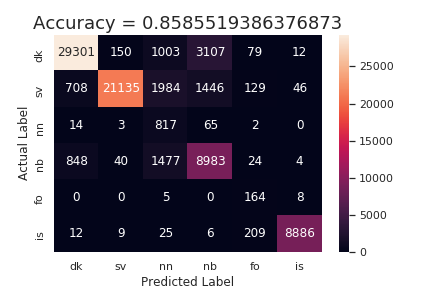
\includegraphics[scale=0.5]{figs/fasttextcharngram}
    \caption{Confusion matrix for FastText trained using only character level n-grams on the Wikipedia data set and evaluated on the Tatoeba data set.}
    \label{fasttextcharngram}
\end{figure}

\begin{figure}
    \begin{subfigure}[b]{0.45\textwidth}
      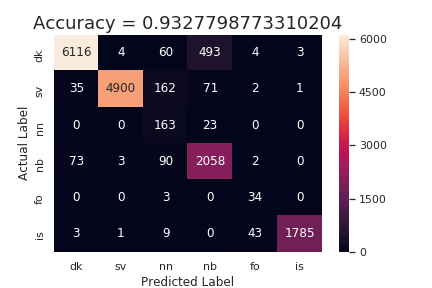
\includegraphics[scale=0.5]{figs/retrain}
      \caption{Confusion matrix for FastText trained using only character level n-grams on the combined Wikipedia/Tatoeba data set and evaluated on the Tatoeba data set.}
      \label{retrain-confuss}
    \end{subfigure}
    ~
    \begin{subfigure}[b]{0.45\textwidth}
        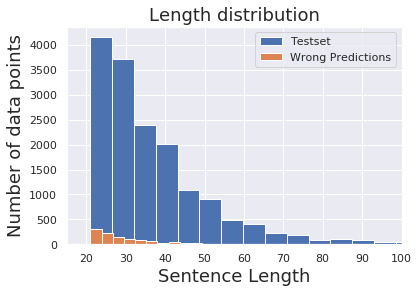
\includegraphics[scale=0.5]{figs/faliurelengthdist_tatoeba}
        \caption{Distribution of sentence lengths Tatoeba test set along with the mis-classified sentences.}
     \label{retrain-lengths}
    \end{subfigure}
    \caption{Error analyses.}
\end{figure}


% In Figure \ref{training} we see a plot of the accuracy during training on the training and validation set respectively. We see that the accuracy on the validation set follows the accuracy on the training set more closely for the CNN than for the MLP.

% \begin{figure}[h!]
%     \centering
%     \begin{subfigure}[b]{200pt}
%         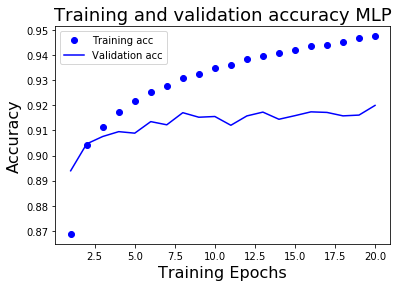
\includegraphics[scale=0.5]{figs/training_MLP}
%         \caption{Training accuracy MLP}
%     \end{subfigure}
%     ~
%     \begin{subfigure}[b]{200pt}
%         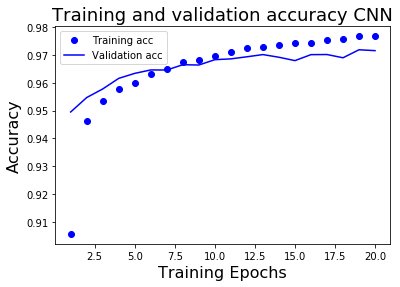
\includegraphics[scale=0.5]{figs/training_CNN}
%         \caption{Training accuracy CNN}
%     \end{subfigure}
%     \caption{Accuracy on test and validation set during training of the different neural networks on the full data set with 50K data points in each language.}
%     \label{training}
% \end{figure}

In Figure~\ref{confusion_matrix-big-cnn} we see the confusion matrix for the convolutional Neural Network trained on the full Wikipedia data set with 300K data points pr language. We see that the largest classification errors still happens between Danish, Bokmål and Nynorsk as well as between Icelandic and Faroese. \\



\subsection{Using FastText supervised}

FastText can also be used for be trained supervised and be used for Classification. In the Paper Bag of Tricks for Efficient Text Classification \cite{BagOfTricks} the authors show that FastText can obtain performance on par with methods inspired by deep learning, while being much faster on a selection of different tasks in Tag prediction and Sentiment Analysis. The confusion matrix from running the FastText supervised classifier can be seen in Figure \ref{fasttext_supervised}. We see that FastText is roughly on par with the CNN.\\

\subsection{Evaluating the models on another data set}
It would be interesting to see how the two best performing models generalize by testing on a data set different from the they have been trained on (the Wikipedia data set).\\

I downloaded an additional data set from Tatoeba\footnote{{\tt tatoeba.org/}} which is a large database of user provided sentences and translations. In Figure \ref{tatoebasentprlang} we see the number of sentences in each language for all sentences in the Tatoeba data set. Observe that we have very few samples in Nynorsk and Faroese.\\

The language used in the Tatoeba data set is different from the language used in Wikipedia. The Tatoeba data set mainly consists of sentences written in everyday language. Below we see some examples from the Danish part of the Tatoeba data set.
\begin{verbatim}
Hvordan har du det?

På trods af al sin rigdom
og berømmelse, er han ulykkelig.

Vi fløj over Atlanterhavet.

Jeg kan ikke lide æg.

Folk som ikke synes at latin er det
smukkeste sprog, har intet forstået.
\end{verbatim}

% The confusion matrix for the FastText supervised model and the CNN, which are both trained on the full Wikipedia data set and then evaluated on the Tatoeba data set can be seen in Figure \ref{tatoeba-confuss}. Both models use the same setting that produced good results on the Wikipedia data set.

% \begin{figure}[h!]
%     \centering
%     \begin{subfigure}[b]{0.45\textwidth}
%         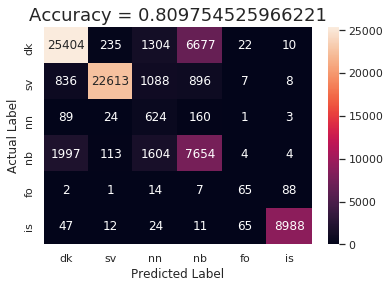
\includegraphics[scale=0.5]{figs/tatoeba-langid}
%         \caption{Langid.py}
%     \end{subfigure}
%     ~
%     \begin{subfigure}[b]{0.45\textwidth}
%         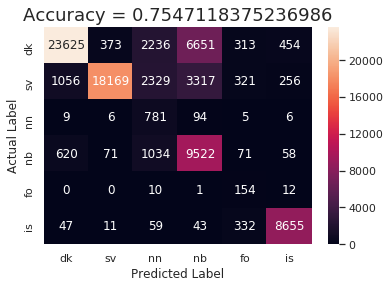
\includegraphics[scale=0.5]{figs/tatoeba-fasttext}
%         \caption{fasttext classifier }
%     \end{subfigure}
%     ~
%     \begin{subfigure}[b]{0.45\textwidth}
%         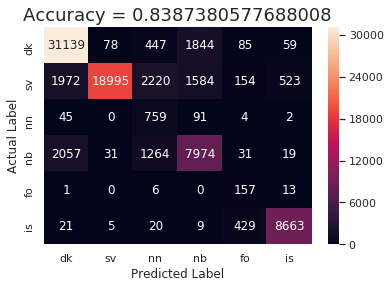
\includegraphics[scale=0.5]{figs/tatoeba-cnn}
%         \caption{Convolutional neural network}
%     \end{subfigure}
%     \caption{Confusion matrices for the tatoeba data set }
%     \label{tatoeba-confuss}
% \end{figure}

We see that the performance drops quite a lot when shifting to another domain. For reference the accuracy of langid.py on this data set is 80.9\% so FastText actually performs worse than the baseline with an accuracy of 75.5\% while the CNN is a bit better than the baseline with an accuracy of 83.8 \% \\

One explanation for the drop in performance is that the sentences in the Tatoeba data set is significantly shorter than the sentences in the Wikipedia data set as seen in Figure~\ref{tatoebalengths}. As we saw in the previous section both models tend to mis-classify shorter sentences more often than longer sentences. This and the fact that the "genre" of sentences are different might explain why the models trained on the Wikipedia data set does not generalize too well to the Tatoeba data set without a drop on performance.\\

The CNN uses character bi-grams as features while, with the standard settings, FastText uses only individual words to train. The better performance of the CNN might indicate that character level n-grams are more useful features for language identification than words alone.\\

To test this we changed the setting of FastText to train using only character level n-grams in the range 1-5 instead of individual words. In Figure \ref{fasttextcharngram} we see the confusion matrix for this version of the FastText model. This version still achieved 97.8\% on the Wikipedia test set while improving the accuracy on the Tatoeba data set from 75.4\% to 85.8\% which is a substantial increase.\\

Thus using character level features seem to improve the FastText models ability to generalize to sentences belonging to a domain different from the one it has been trained on.\\


\subsection{Retraining on the combined data set}
To improve the accuracy over the Tatoeba data set we retrained the FastText model on a combined data set consisting of data points from
both the Wikipedia and Tatoeba data set.\\

The FastText model achieved an accuracy of 97.2\% on this combined data set and an accuracy of 93.2\% when evaluating this model on the Tatoeba test set alone - the confusion matrix can be seen in Figure \ref{retrain-confuss}.\\

As was the case with the Wikipedia data set the mis-classified sentences tend to be shorter than the average sentence in the data set. In Figure \ref{retrain-lengths} we see the distribution of sentence lengths for the Tatoeba test set along with the mis-classified sentences.\\

In the Tatoeba test set the mean length of sentences is 37.66 characters with a standard deviation of 17.91 while the mean length is only 29.70 characters for the mis-classified sentences with a standard deviation of 9.65. This again supports the conclusion that shorter sentences are harder to classify.\\

